% 6_algoritmo.tex

% Un diagrama de flujo del algoritmo de la solución propuesta.
\section{Algoritmo propuesto}

Para implementar el comportamiento deseado, se propone utilizar los algoritmos mostrados en las Figuras \ref{fig:flowchart-tx} y \ref{fig:flowchart-rx}.
A diferencia de un diseño simétrico, en esta solución cada dispositivo tiene un rol fijo: uno actúa exclusivamente como transmisor y el otro exclusivamente como receptor.

El nodo transmisor, cuyo flujo se ilustra en la Figura \ref{fig:flowchart-tx}, permanece en espera hasta que el usuario presiona el botón de inicio.
Al detectarse dicha pulsación, el dispositivo realiza la grabación y transmisión del audio.
Al finalizar, el nodo regresa al estado de espera, listo para una nueva transmisión.

\begin{figure}[htbp]
    \centering
    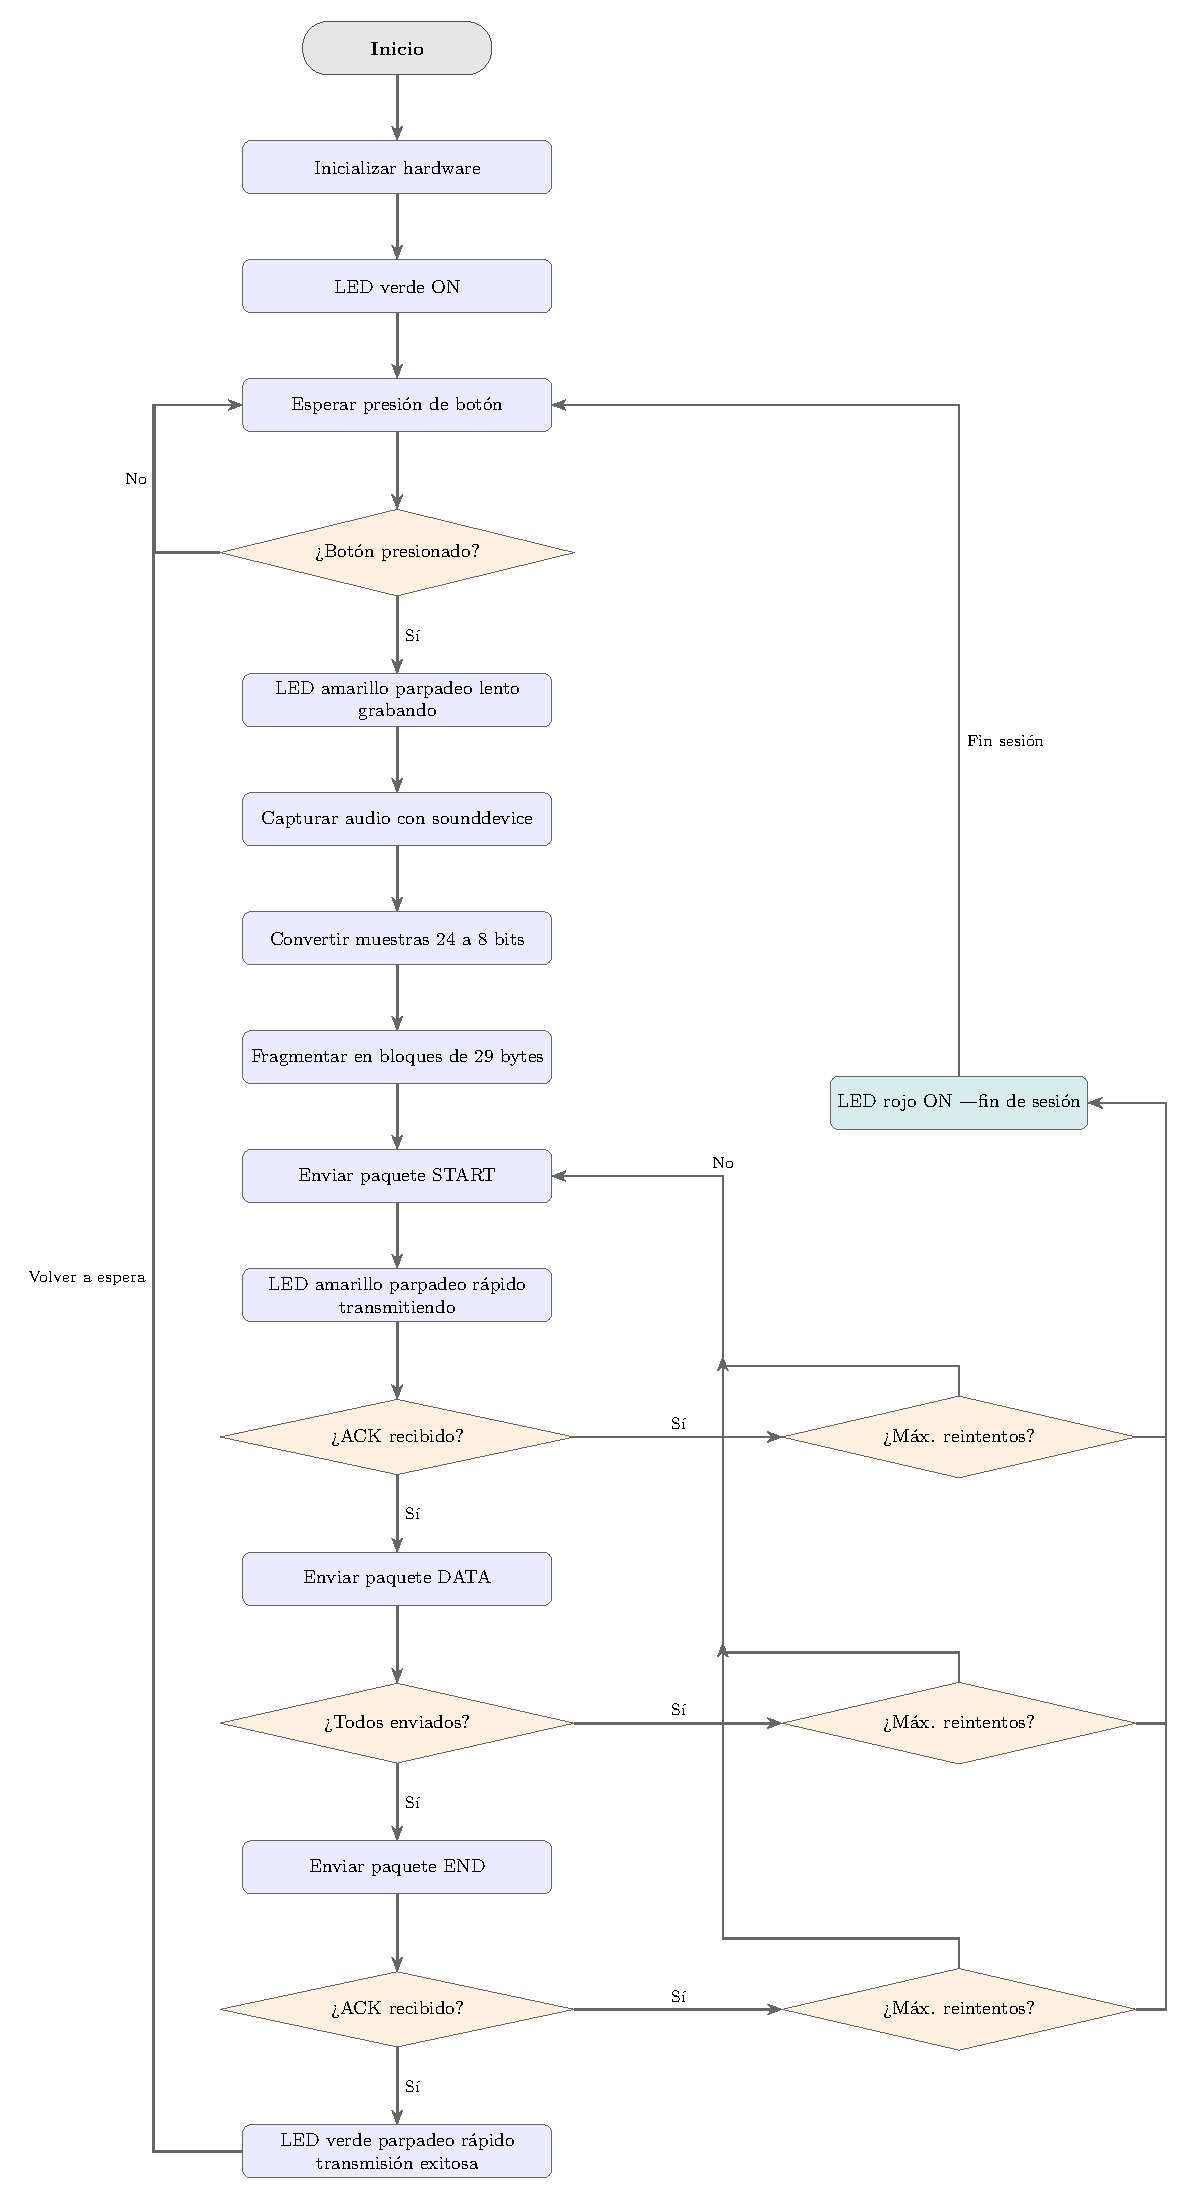
\includegraphics[width=0.67\textwidth]{images/fc_tx.pdf}
    \caption{Diagrama de flujo del nodo transmisor.}
    \label{fig:flowchart-tx}
\end{figure}

El nodo receptor, por su parte, permanece continuamente en modo de recepción a la espera de un \texttt{START} que señale el inicio de una transmisión (este diseño se especifica en la sección \ref{sec:organizacion_transferencia}).
Al recibirlo, gestiona la recepción y reproducción del audio, como se ilustra en la Figura \ref{fig:flowchart-rx}.
Una vez finalizado, el nodo regresa al estado de espera para atender una nueva transmisión.

\begin{figure}[htbp]
    \centering
    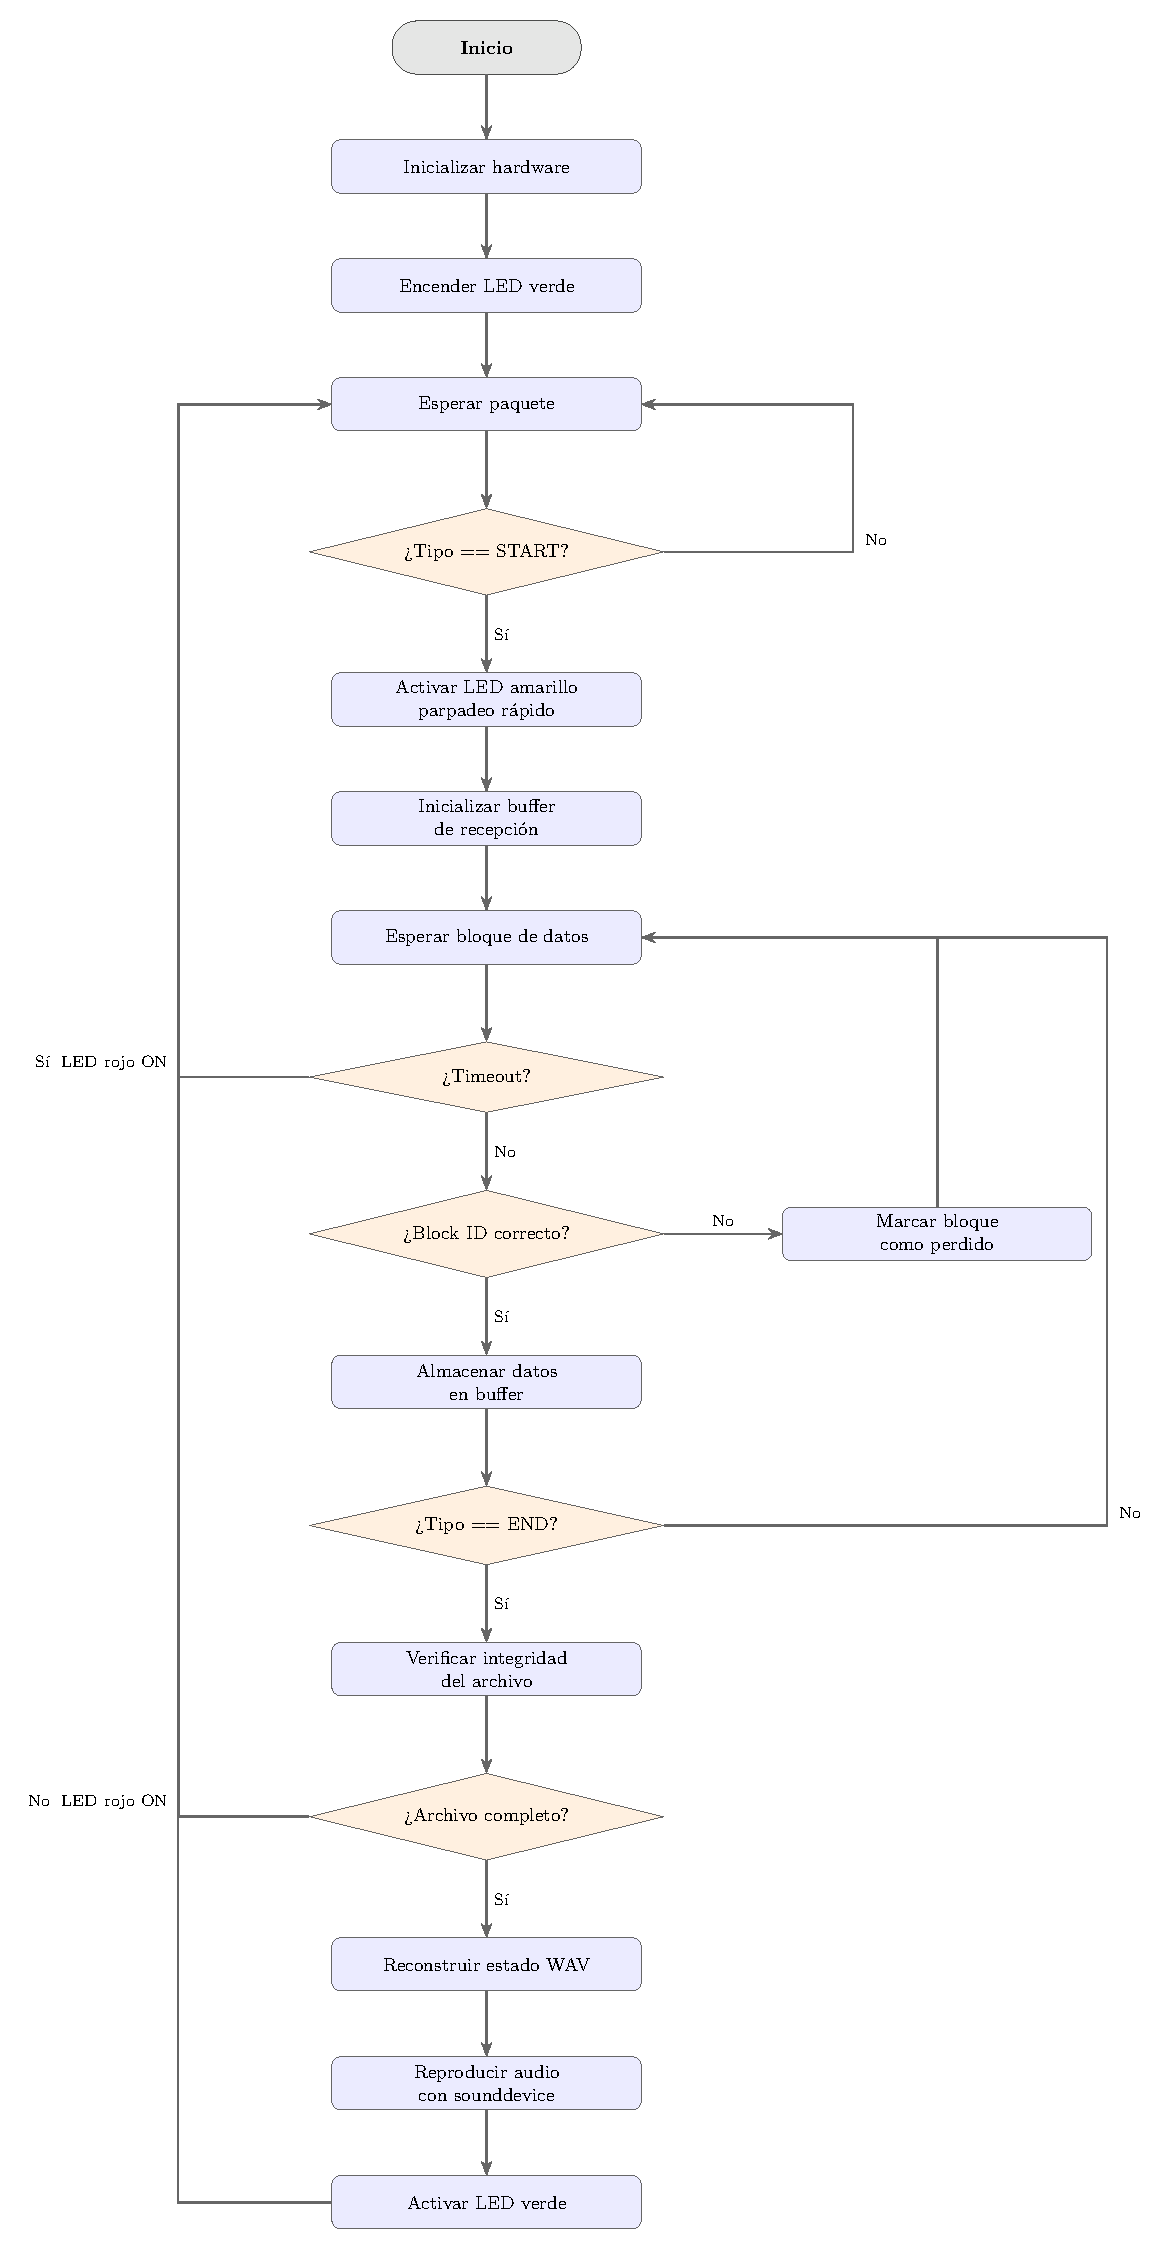
\includegraphics[width=0.65\textwidth]{images/fc_rx.pdf}
    \caption{Diagrama de flujo del nodo receptor.}
    \label{fig:flowchart-rx}
\end{figure}

Por simplicidad, no se considerará el caso en que el botón de transmisión se presione durante un proceso de transmisión o reproducción en curso.
Se asume que el botón únicamente se acciona una vez transcurrido un tiempo suficiente para completar el proceso anterior.
De no cumplirse esta condición, no se garantiza el funcionamiento correcto del sistema.

La comunicación inalámbrica entre dispositivos se realizará mediante el protocolo \textit{Enhanced ShockBurst} (ESB), que se detalla en la siguiente sección.

Adicionalmente, el tipo de compresión de audio es seleccionable en el nodo transmisor mediante configuración.
Se puede elegir entre PCM lineal de $8$ bits y ADPCM.
El códec seleccionado se indica en el paquete \texttt{START}, de modo que el nodo receptor lo detecta automáticamente y aplica la decodificación correspondiente sin requerir reconfiguración manual.

Se usarán tres LEDs para indicar al usuario el estado del sistema durante la captura, transmisión, recepción y reproducción según el código mostrado en la Tabla \ref{tab:led_states}.

\begin{table}[htb]
\centering
\begin{tabular}{lccc}
\toprule
Estado & LED verde & LED amarillo & LED rojo \\
\midrule
Listo / espera      & Encendido & Apagado         & Apagado   \\
Grabando            & Apagado   & Parpadeo lento  & Apagado   \\
Transmitiendo       & Apagado   & Parpadeo rápido & Apagado  \\
Recibiendo          & Apagado   & Parpadeo rápido & Apagado  \\
Error               & Apagado   & Apagado         & Encendido \\
Transmisión exitosa & Parpadeo rápido & Apagado   & Apagado   \\
Reproduciendo       & Encendido & Encendido       & Apagado   \\
\bottomrule
\end{tabular}
\caption{Estados de los LEDs.}
\label{tab:led_states}
\end{table}

Como alternativa de diseño, una forma más elegante de resolver el presente problema es a partir de una máquina de estados finita tanto para el nodo transmisor como el receptor.
En las Figuras \ref{fig:fsm_tx} y \ref{fig:fsm_rx} se muestran los diagramas de estados planteados para cada una, respectivamente.
Este diseño permite modelar el comportamiento del hardware utilizado de forma sencilla y facilita la programación y \textit{debugging}, en comparación con una lógica condicional extensa.
Este es el que finalmente se implementó, donde tanto el nodo transmisor como el receptor se programaron como máquinas de estado.
Entonces, los diagramas de flujo mostrados anteriormente permiten entender el comportamiento requerido y con los diagramas de estados se resume el planteamiento ideado a nivel de código.
Este fue el diseño implementado.

\begin{figure}[htbp]
    \centering
    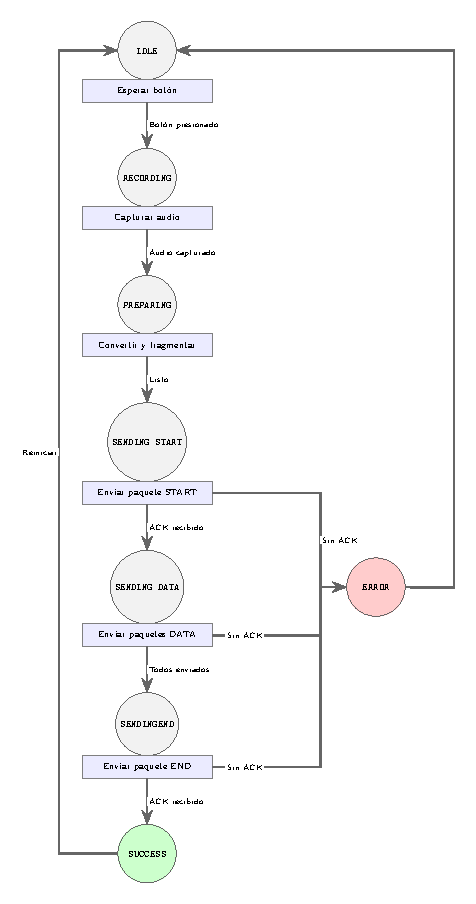
\includegraphics[width=0.65\textwidth]{images/fsm_tx.pdf}
    \caption{Diagrama de estados del nodo transmisor.}
    \label{fig:fsm_tx}
\end{figure}

\begin{figure}[htbp]
    \centering
    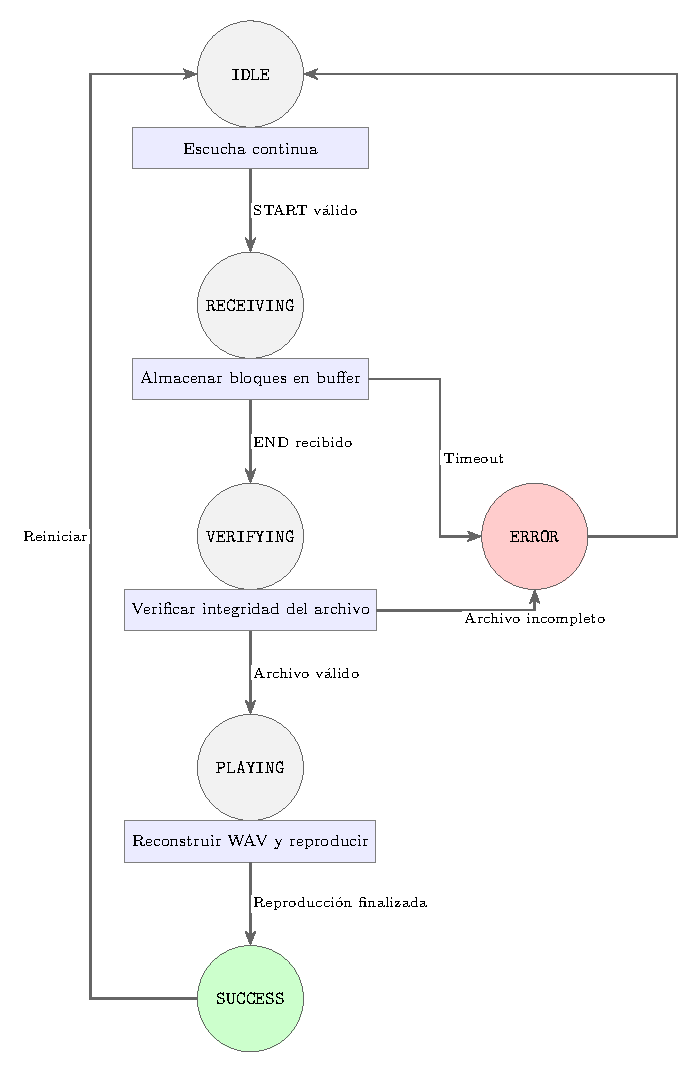
\includegraphics[width=0.65\textwidth]{images/fsm_rx.pdf}
    \caption{Diagrama de estados del nodo receptor.}
    \label{fig:fsm_rx}
\end{figure}